% !TeX spellcheck = it_IT

%Roba nuova, introduci

\section{Algoritmi Distribuiti}

In un ambiente di calcolo distribuito, possiamo pensare alle entità di calcolo come nodi all'interno di un \textbf{grafo direzionato} $\vec G$, dove ogni arco indica un collegamento.\\

Ogni \textbf{entità possiede}:
\begin{itemize}
	\item Memoria locale
	\item Capacità di calcolo 
	\item Capacità di comunicazione
	\item \textbf{Clock locale}
\end{itemize} 

La differenza dal capitolo precedente è che i \textbf{processori sono asincroni}.\\

Nella memoria locale abbiamo: 
\begin{itemize}
	\item Registro di \textbf{input}: \texttt{valore($x$)}, input dell'entità $x$
	\item Registro di \textbf{stato} $=$ \texttt{stato($x$)}, stato dell'entità $x$; questo valore può essere cambiato localmente dalla stessa $x$
\end{itemize}

Per il \textbf{clock locale} è possibile settare o resettare una \textbf{sveglia}.\\
 \newpage

\paragraph{Proprietà delle entità:}
\begin{enumerate}
	\item \textbf{Reattive:} all'accadere di un "evento" compiono un'azione. Gli eventi possono essere:
	\begin{itemize}
		\item \textbf{Interni} al sistema: ricezione di messaggi, sveglia
		\item \textbf{Esterni} al sistema: impulso spontaneo (impulso di start)
	\end{itemize}
	L'entità sollecitata dall'evento risponde con un'azione: una \textbf{sequenza finita di operazioni indivisibili} (deve arrivare al termine).\\
	
	\item \textbf{Le entità seguono delle regole:} una \textbf{regola} è un oggetto della \textbf{forma} \texttt{stato $\times$ evento $\rightarrow$ azione}.\\
	Sia $x$ un'entità, allora $B(x)$ è l'\textbf{insieme delle regole a cui è soggetta} $x$. $B(x)$ deve essere \textbf{completo} (ogni coppia stato-evento deve avere un'azione specificata) e \textbf{non ambiguo} (con una singola interpretazione possibile).\\
	
	Se $E$ è un'\textbf{insieme di entità} che collaborano tra loro allora $B(E)$ è il \textbf{comportamento del sistema}
	$$ B(E) = \bigcup_{x \in E} B(x) $$
	è importante che $E$ sia \textbf{omogeneo}:
	$$ \forall x,y \in E, \;\;\;\;\; B(x) = B(y)$$
	Quando $B(E)$ è omogeneo viene chiamato \textbf{protocollo} per $E$ o \textbf{algoritmo distribuito} per E.\\
\end{enumerate}

\paragraph{Fact:} Sempre possibile ottenere $B(E)$ omogeneo.\\

\begin{proof}
	L'idea è di utilizzare un registro locale aggiuntivo che \textbf{differenzia} quelle \textbf{entità} che alla \textbf{stessa coppia stato-evento hanno azioni diverse}. Si usa
	\begin{itemize}
		\item \texttt{ruolo($x$)}: registro locale di $x$ che contiene il ruolo per $x$
	\end{itemize}
	
	La regola diventa:  \\
	\begin{tabular}{c c}
			\texttt{stato} $\times$ \texttt{evento} $\rightarrow$ \texttt{If ruolo(x)} & \texttt{then} $A_a$ \\ 
			& \texttt{else} $A_b$
	\end{tabular}
	\nn
\end{proof}

\newpage

\paragraph{Proprietà della rete: }
\begin{enumerate}
	\item La \textbf{comunicazione} tra entità \textbf{avviene usando link}, ed è importante che ogni entità conosca i propri collegamenti. Per ogni entità $x$, si ha un \textbf{etichettatura} denotata con $\lambda_x$ e dato che si trova in $\vec G$, si indicano con: 
	\begin{itemize}
		\item $N_{in} (x) =$ vicini in \textbf{ingresso} ad $x$
		\item $N_{out} (x) =$ vicini in \textbf{uscita} da $x$
	\end{itemize}
	
	\begin{center}
		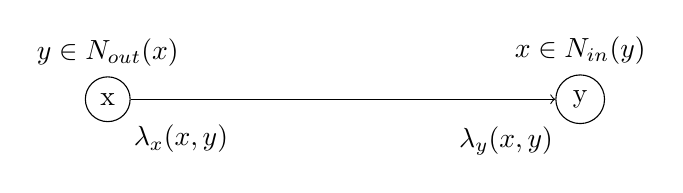
\begin{tikzpicture}
					\node[circle, draw, label=90:{$y \in N_{out} (x)$}, label=315:{$\lambda_x (x,y)$}] (x) at (0,0) {x}; 
					\node[circle, draw, label=90:{$x \in N_{in} (y)$}, label=225:{$\lambda_y (x,y)$}] (y) at (6,0) {y}; 
					\draw[->] (x) -- (y);
		\end{tikzpicture}
	\end{center}
	
	Per $x$ la funzione sarà $\lambda_x (x,y)$, mentre per $y$ l'etichettatura sarà $\lambda_y (x,y)$.\\
	
	\item \textbf{Assiomi di rete: }
	\begin{itemize}
		\item \textbf{Ritardo finito di comunicazione:} in assenza di errori, un messaggio spedito prima o poi arriverà
		\item \textbf{Orientamento locale:} ogni entità riesce a distinguere tra i suoi vicini $N_{in} (x)$ e $N_{out} (x)$ grazie alla conoscenza della funzione $\lambda_x$
	\end{itemize}
	\nn
\end{enumerate}

\paragraph{Parametri di rete: }
\begin{itemize}
	\item \textbf{Numero} di \textbf{entità} $n$ (nodi).\\
	
	\item \textbf{Numero} di \textbf{link} $m$ (archi).\\
	
	\item \textbf{Diametro} della rete $d$ (massima distanza tra due nodi).\\
\end{itemize}

\newpage

Oltre agli assiomi possiamo avere delle \textbf{restrizioni sulla rete}, da dichiarare al momento della scrittura del codice. Generalmente sono proprietà positive della rete, su cui fare affidamento.\\

\paragraph{Restrizioni sulla comunicazione:} 
\begin{itemize}
	\item \textbf{Link bidirezionali:} le connessioni tra le entità sono full duplex, si passa da un grafo diretto ad uno non diretto..\\
	$\forall x$, $N_{in} (x) = N_{out} (x) = N(x)$, quindi anche $\lambda_x (x, y) = \lambda_x (y, x)$.\\
	
	\item \textbf{Ordinamento dei messaggi:} i messaggi sullo stesso link vengono prelevati con politica FIFO (il primo inviato è il primo ad arrivare)
\end{itemize}

\paragraph{Restrizioni sull'affidabilità: }
\begin{itemize}
	\item \textbf{Rilevazione di errori:} ad esempio, quando cade un'entità o si guasta un canale di comunicazione.\\
	
	\item \textbf{Affidabilità parziale:} non ci saranno errori in futuro.\\
	
	\item \textbf{Affidabilità totale:} non ci sono stati errori e non ce ne saranno in futuro.\\
\end{itemize}

\paragraph{Restrizioni sulla topologia di rete: }
\begin{itemize}
	\item \textbf{Connettività del grafo:} $\vec G$ è fortemente connesso, $G$ è connesso.\\
\end{itemize}

\paragraph{Restrizioni sul tempo: }
\begin{itemize}
	\item \textbf{Tempi di comunicazione unitari:} la comunicazione impiega sempre un singolo ciclo di clock.\\
	
	\item \textbf{Clock sincronizzati:} come fosse un'architettura parallela a memoria distribuita.\\
\end{itemize}

\textbf{Nota:} tali restrizioni a volte vengono considerate per il calcolo delle prestazioni \textbf{ideali} del codice distribuito.\\

\newpage

%Slide 11
%End L19